\documentclass[12pt]{article}

\usepackage{upgreek}

\usepackage{amsmath}

\usepackage{graphicx}

\usepackage{dsfont}

\usepackage{hyperref}

\usepackage[utf8]{inputenc}

\usepackage{graphicx}
\graphicspath{ {imgs/} }

\usepackage{mathtools}

\usepackage{textcomp}

\usepackage[english]{babel}

\usepackage{tikz}

\usepackage{tcolorbox}

\usepackage{amsthm,amssymb}

\setlength{\parindent}{0cm}

\renewcommand\qedsymbol{$\blacksquare$}

\usepackage{fancyhdr}
 
\pagestyle{fancy}
\fancyhf{}
\fancyhead[LE,RO]{Introduction to Databases -- Fall 2017}
\fancyhead[RE,LO]{Joshua Concon}
\fancyfoot[CE,CO]{\leftmark}
\fancyfoot[LE,RO]{\thepage}


\begin{document}

\title{CSCC43: Introduction to Databases\\ Lecture Notes}
\date{University of Toronto Scarborough -- Fall 2017}
\author{Joshua Concon}
\maketitle
Pre-reqs are CSCB63 and STAB52.
Instructor is Dr. Marzieh Ahmadzadeh. Check RateMyProf. If you find any problems in these notes, feel free to contact me at conconjoshua@gmail.com.

\tableofcontents

\pagebreak

\section{Thursday, September 7, 2017}

\subsection{Definitions}

\paragraph{Data} Objects or events that could be recorded on a computer media. This includes stuff like an email, an address, a student identification number, etc.\\

However, there are two types of Data, Unstructured and Structured.

\paragraph{Structured Data} They are mostly stored in a tabular format, have types including: date, character, numeric, alphanumeric.

\paragraph{Unstructured Data} Data that must be analyzed to extract information from, does not already show information. Includes multimedia, maps, documents, pictures, voices.

\paragraph{Database} An organized collection of logically related data that can be of any size or complexity. Example:
\begin{itemize}
	\item{Student ID, name, GPA, courses taken}
	\item{Patient name, doctor's ID, ward, date of admission}
	\item{Personnel ID, base salary, bonus, hours of work}
\end{itemize}

\underline{Another Example:}

\begin{center}
 \begin{tabular}{||c c c||} 
 \hline
 ID & Course & Mark \\ [0.5ex] 
 \hline\hline
 100 & CSCC43 & A \\ 
 \hline
 100 & CSCC44 & B \\
 \hline
 100 & CSCC52 & A+  \\
 \hline
 200 & CSCC43 & A+\\
 \hline
 200 & CSCC62 & B\\ [1ex] 
 \hline
\end{tabular}
\end{center}

\paragraph{Database Management System (DBMS)} A software that sits between users and databases, responsibilities include:
\begin{itemize}
	\item{Allowing users to create, update, sort or retrieve data}
	\item{Enforcing the integrity of data (consistency, etc.)}
	\item{Improving performance when dealing with huge data or many queries}
	\item{Assuring the durability of the data}
	\item{Allowing data to be shared among different programs}
	\item{managing concurrent access by multiple users/processes}
\end{itemize}

\paragraph{Information} Information is data that has been process in order to increase user knowledge, could be data provided in a way that can be analyzed easily (i.e. has labels, maybe graphs showing relationships, etc.)

\paragraph{Metadata} "Data about data". Data that describes the properties of end-user data and it's context, it helps the database designer understand what kind of data exists and what it means. Examples include name, type, length, allowable values, ownership (stewardship), source...
\\
\underline{Example:}\\
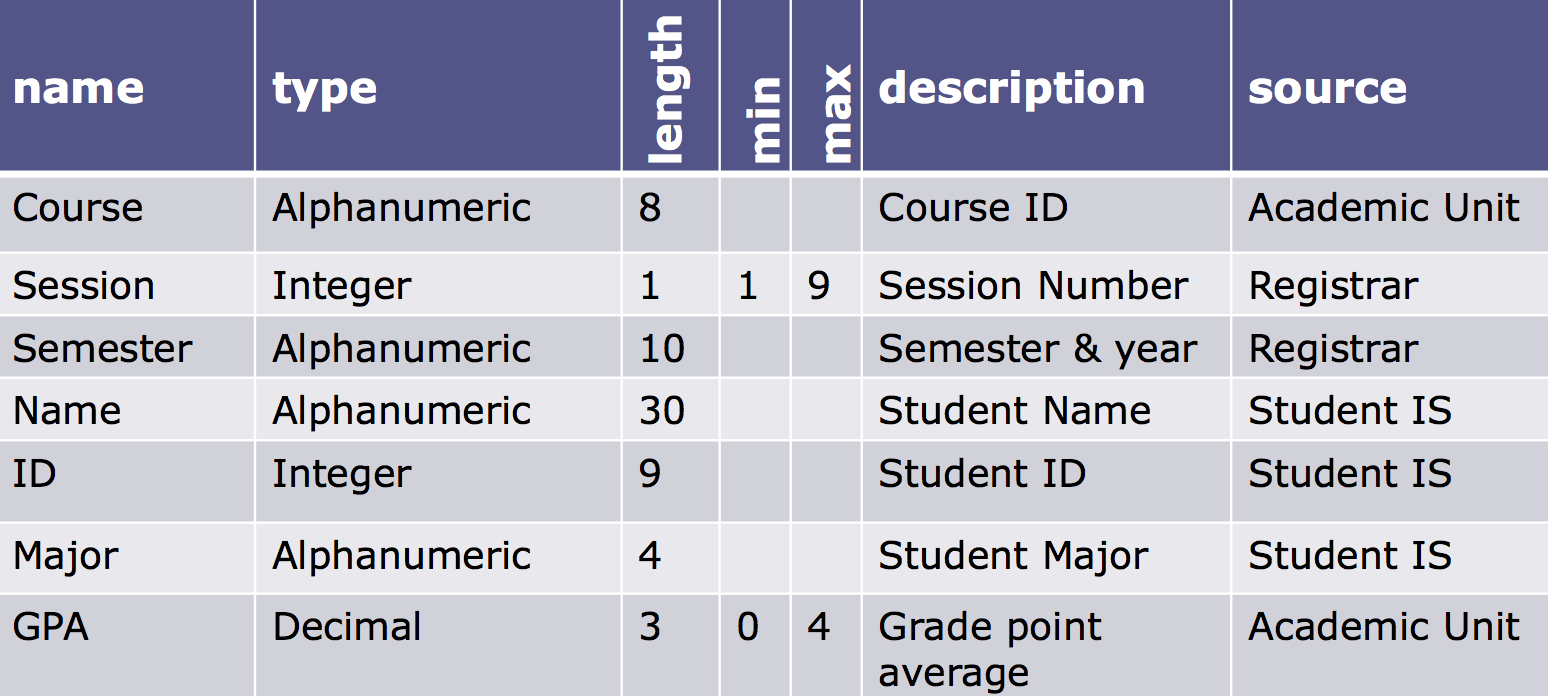
\includegraphics[scale=0.5]{lec1-1}

\subsection{How do we store data?}

There are two ways we can store data, either the Traditional file system or the database approach.

\subsubsection{Traditional File System}

The Traditional File System includes files that are also collections of related data, was used prior to the invention of databases, but has its own disadvantages.\\
\\
\underline{Example of a file system:}\\
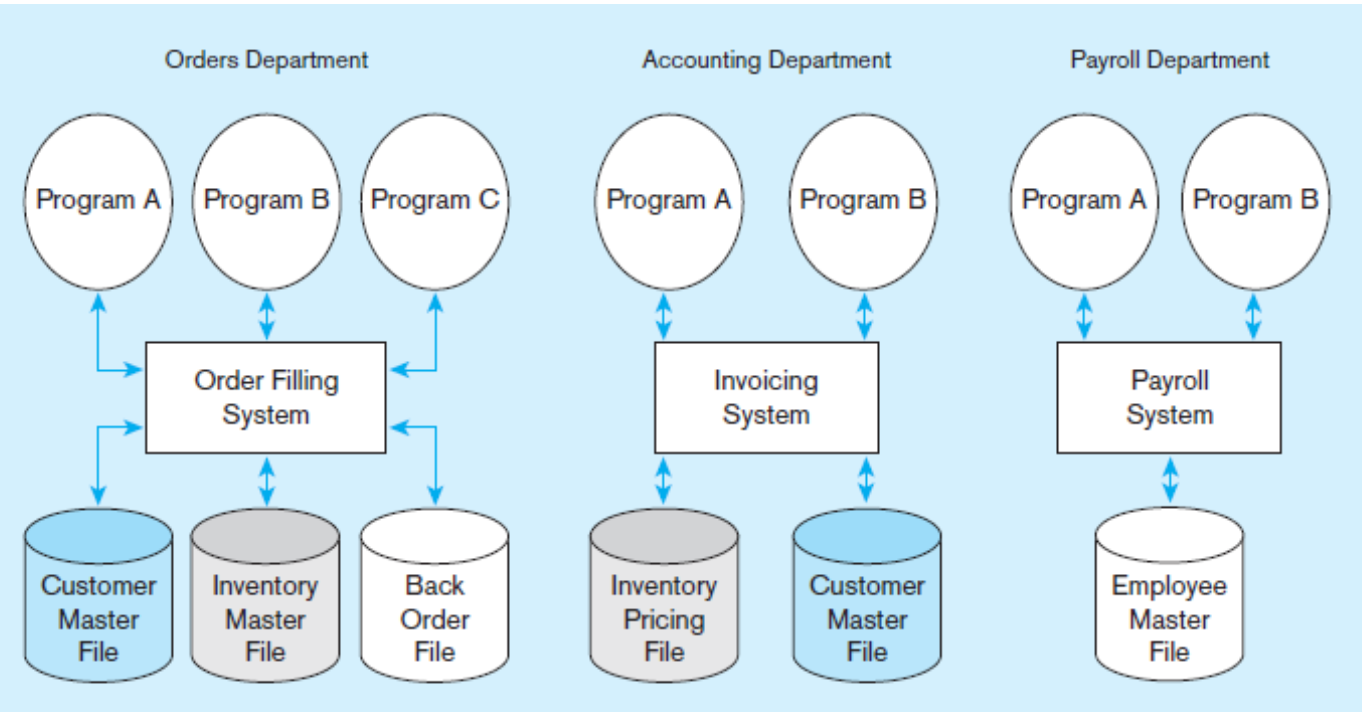
\includegraphics[scale=0.5]{lec1-2}\\

\underline{Disadvantages:}
\paragraph{Program-Data Dependence} If the data is changes, all programs that used the data should be altered to. To use an example from the previous image, if the length of data such as customer name is changed, order filling system programs and invoice system programs are both affected. Using the database approach, this is managed by a Database Management System and no change in order filling or account programs are required, only on the file itself.

\paragraph{Duplication of Data} As seen from the last image, the order filling system and the invoice system both have a customer master file. This is a waste of space as it is essentially two sets of the same data, and reliable metadata is difficult to establish since it may be inconsistent. Changes to one copy must also be applied to the other, so this may compromises the files' data integrity.

\paragraph{Limited Data Sharing} Since each application has its own data, data sharing between applications is not easy, a system does not have access to another system's data. With the database approach, data sharing is doable.

\paragraph{Length Development Times} Each new application should be started from scratch by designing a new file format and description, however, in the database approach, you only need to design your database once, and can easily access the data you need.

\paragraph{Excessive Program Maintenance} All preceding factors creates heavy program maintenance, so to avoid these disadvantages, the database approach is preferred. Note that if a database is not properly designed, mentioned disadvantages may not disappear.

\subsubsection{Database Approach}

The database approach creates a repository of shared data, data is managed by a controlling agent (Database Management System), and all data is stored in a standardized convenient form.\\
\\
\underline{Visualization Example:}\\
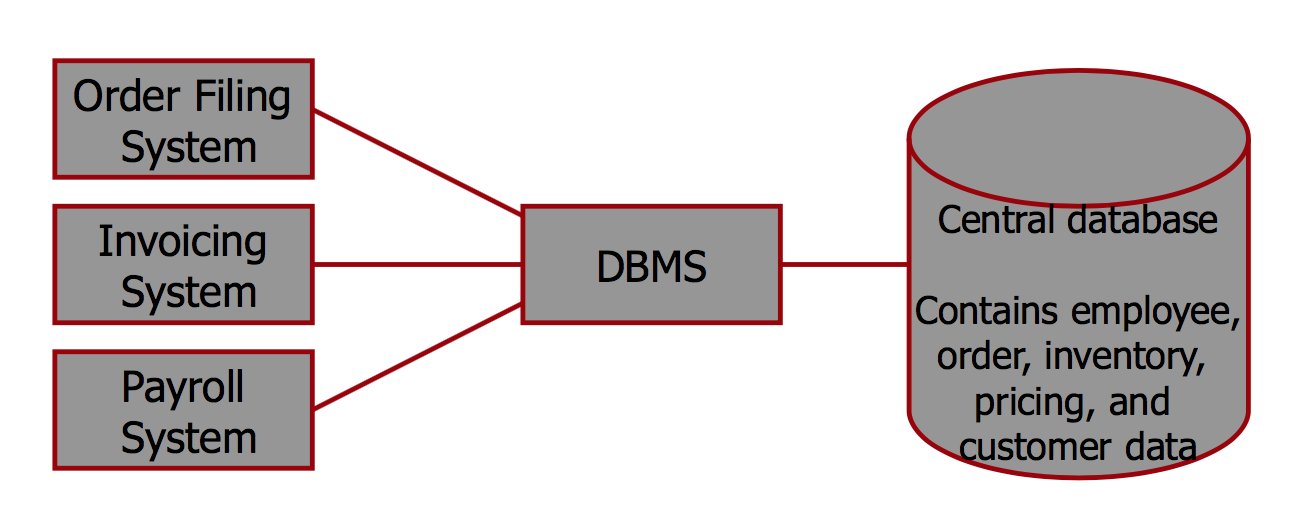
\includegraphics[scale=0.5]{lec1-3}\\

Every Database uses a data model, and this data model is a notation for describing data that specifies the structure of the data, the constrains on the content of the data, and the operations on the data.\\
\\
Some examples of data models include a relational data model, a semistructured data model, unstructured data, and an Object-oriented model.

\subsection{Relational Data Model}

The main concept of the relational data model is a relation, which is based off the concept of relations in math. A relation in a database is like a table consisting of rows and columns.\\
\\
\underline{Example:}\\
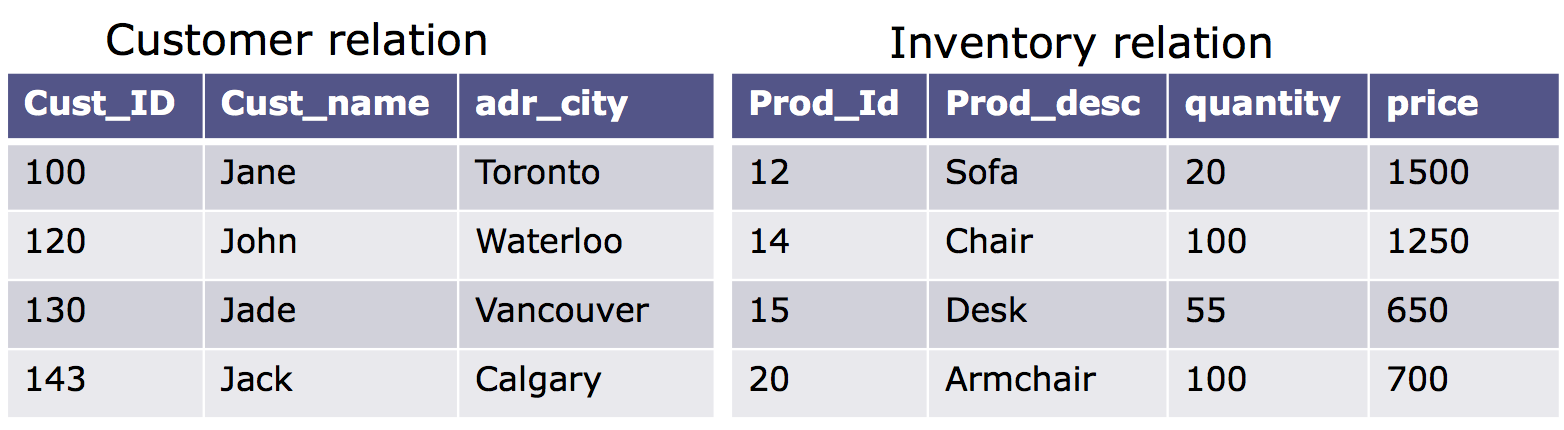
\includegraphics[scale=0.5]{lec1-4}\\

\subsubsection{Advantages}

\paragraph{Program-data independence} Metadata is stored in a central location called a repository, and data could be changed independent of what program uses it.

\paragraph{Planned data redundancy} Data is only duplicated when we want it to be duplicated, so we can control redundancy.

\paragraph{Improved data consistency} Which is implied since data redundancy is eliminated.

\paragraph{Increased productivity of application development} Since the application does not deal with the data management, since it is taken care of by the Database Management System, so time and cost of development is saved.

\paragraph{Enforcement of standards} Standards are enforced by the uniform procedures for accessing and updating data.

\paragraph{Improved data quality} By defining constraints that the data must follow.

\paragraph{Improved data accessibility and responsiveness} Can be done by using a query system to access data.

\paragraph{Reduced program maintenance} Because of data-program independence, changing the data does not affect any program.

\paragraph{Improved data sharing} By creating a user view and since all applications share the same data already, data sharing is doable.

\subsubsection{Cost and Risk}

\paragraph{New specialized personnel} Companies need to hire new people for database design and database administration services.

\paragraph{Installation and Management of Cost and Complexity} Implementation of the database and scaling it will be a new concern for companies

\paragraph{Conversion Costs} Costs for converting legacy system to a modern database

\paragraph{Need for backup and recovery} New costs and concerns for backing up the database and new services companies must worry about for recovery.

\paragraph{Organizational Conflict} On data definition, data format and right to update data.

\subsection{Database Development Process}

\paragraph{Model the rule of the organization} Such as, "each student at UofT can take up to 5 courses in one semester"

\paragraph{Explore a relation between various entities} Such as, "A course might be taken by many students", "A student must take at least one course", etc.

\paragraph{Create your relation} Creating the tables with relations between the entities and data associated with each object

\paragraph{Normalize your relation} We will learn what this is later in the course

\paragraph{Implementation} Actual Implementation of the database

\newpage

\end{document}


























